\documentclass{aaa}
\usepackage[urlcolor=blue]{hyperref}
\usepackage{threeparttable}
\usepackage{setspace}
\usepackage{titlesec}
\usepackage{float}
\usepackage{makecell}
\usepackage{graphicx}
\usepackage{epstopdf}
\usepackage{listings}
\usepackage{booktabs}
\usepackage{indentfirst}
\usepackage{multirow}
\graphicspath{ {figure/} } 
\newcommand{\upcite}[1]{\textsuperscript{\textsuperscript{\cite{#1}}}}
\usepackage{fancyhdr}
\titleformat{\section}{\large \heiti}{\chinese{section}、}{0em}{}

\makeatletter
\newcommand{\figcaption}{\def\@captype{figure}\caption}
\newcommand{\tabcaption}{\def\@captype{table}\caption}
\makeatother
\setlength{\parindent}{2.45em}

\begin{document}
\begin{center}
\LARGE
  \textbf{文献整理:改进的光学大气质量表及其近似公式}\\
  \vspace{0.2em}
  \large
    杜沈达 \\%\ 学号:2016xxxxxx \\ %姓名,学号,班级
  安光所遥感中心
  \end{center}
\rule[0.1\baselineskip]{\textwidth}{0.5pt}
\textbf{简 \ 介}\\
\large
整理的文献为"Revised optical air mass tables and approximation formula"。

文章一开始介绍了一个由Karsten在1965年发表的并且广泛被世界所采用的关于大气质量的近似公式,并且讨论了一些由于各个学科对于不同的物理量符号和术语的不同使得读者经常由此而困惑。

其后介绍了一个计算大气光学质量的近似公式,然后说明了在公式中存在的一种不定情况,之后又对这个近似公式用非线性最小二乘法进行修正得到了一组新的系数。后面又根据索引文献\upcite{bib:one}文中也多次提到这篇文献,很多都是从这篇文献里面来的。
\\
%\textbf{关键词}:厚德\quad 笃学\quad 崇实\quad 尚新\\
\rule[0.1\baselineskip]{\textwidth}{0.5pt}
\section{引入一个通用计算公式}
\begin{equation}
	m(\gamma)=\frac{m_{abs}(\gamma)}{m_{abs}(90^{\circ})}
\end{equation}
\begin{equation}
	m_{abs}(\gamma)=\rho_{0}\int^{\infty}_{0} \frac{\rho}{\rho_{0}}([1-[1+2\delta_{0}(1-\frac{\rho}{\rho_{0}})]]\times
	[\frac{\cos \gamma}{1+\frac{h}{R}}]^{2})^{-\frac{1}{2}}dh
\end{equation}
	$h$是相对于海平面的平均高度;\\
	$\rho=\rho(h)$,是在高度$h$处的大气质量;\\
	$\delta_{0}=n_{0}-1$;\\
	$n_{0}$是在$h=0$时对于波长为$0.7\mu m$的空气的折射率;\\
	$R$是地球的平均半径。
	
其中,计算的$m_{abs}(\gamma)$是绝对光学质量,$m(\gamma)$是相对光学质量,在这个式子里面,一些常量是已知的,文献中已经提到,如表1所示。
\begin{center}
	\tabcaption{已知参数表}
	\begin{tabular}{|c|c|c|}
		\hline 
		参数&符号      &值  \\ \hline
		在$h=0$处的大气密度&$\rho_{0}$&$1.22500kg/m^{3}$\\ \hline
		$n_{0}-1$&$\delta_{0}$&$2.76\times 10^{-4}$\\ \hline
		地球平均半径&$R$	&$6.371229\times 10^{6}m$\\ \hline
	\end{tabular}
\end{center}

根据以上的式子(1),(2)和已知的参数表1。要计算这个定积分,那就还需要知道$\rho$,也就是$\rho(h)$在高度$h$处的大气密度,但是我在文献中找不到,这是个问题,不知道是不是需要再去别的地方找这个$\rho$,看完了这篇文章之后,知道了这个$\rho$还是没有找到,但是文章已经给出了计算得到的结果的表格。
\section{近似计算公式和不同的系数}
\begin{equation}
	f(\gamma)=[\sin \gamma+a(\gamma+b)^{-c}]^{-1}
\end{equation}
$\gamma$是天顶角,单位是$^\circ$;\\
$f(\gamma)$是用近似公式计算的$m(\gamma)$;\\
$a,b,c$是式子的常数,$a=0.1500$,$b=3.885^{\circ}$,$c=1.253$;

$a,b,c$这三个常数决定于最小二乘法的相对误差,也就是用前面的计算公式计算数据之后,用最小二乘法进行拟合,使用(3)的形式来计算三个常数。

文献后面又介绍了两个不同的参数组合,一个是根据非线性最小二乘法计算的$a=0.50572,b=6.07995^{\circ},c=1.6364$;一个是根据Bemporad的经典大气质量表确定的,$a=0.6556,b=6.379^{\circ},c=1.757$\upcite{bib:one},其中文献的表中的$r(\gamma)$是根据公式(4)计算的相对误差,用来衡量计算大气质量的相对误差。
\begin{equation}
	r(\gamma)=\frac{f(\gamma)-m(\gamma)}{m(\gamma)}
\end{equation}
\section{积分问题和解决}
对于公式(2),积分会在$\gamma=0$和$h$接近于0的地方不定,在这种情况下,这个积分可以通过执行一个特殊的程序来进行计算,在参考文献\upcite{bib:one}中有写这个程序。但是在计算的时候有个错误会混入,在地平线上的值36.2648会比实际的小5\%左右。

举例而言,在Link和Neuzil\upcite{bib:three}文章的表中所给出的地平线上的在1962年美国的标准大气的大气质量是38.16,这跟1959年Karsen用的ARDC模型十分接近。Snider和Goldman\upcite{bib:four}给出的关于1962年的模型的38.10也是高度相似。Treve\upcite{bib:five}使用1959年的ARDC模型,得到了在地平线上的相对大气质量分别是$0.55\mu$m的38.11和在$0.70\mu$m的38.08。

还有就是采用一种新的标准来却确定式子(2)中的参数会优于旧的模型,也就是最新的国际标准化组织的大气模型(ISO Standrad Atmophere)代替ARDC模型大气(由国际民航组织ICAO提出的),这个仅有的变化也就是名义地球半径变为$R=6.356766\times10^{6}$m。
\section{我要做的工作}
在这篇文章里面,我要做的就是编写一个程序,根据文献中的大气质量近似公式(3),并且用不同的参数组带入,将表格中自变量太阳高度角$\gamma$作为自变量带入近似公式计算,再与表格中所给的大气质量数进行作差比较,即验证这个算法是否真的符合实际,如果误差较小,则可以用到我们的项目中去。
\begin{center}
	\tabcaption{在计算光学质量时候所用的太阳高度角的步长$\Delta \gamma$}
	\begin{tabular}{cc}
		\Xhline{2pt}
		$\gamma$的取值范围($^\circ$)&$\Delta \gamma$ ($^\circ$) \\
		\Xhline{1pt}
		0-20 & 0.1\\
		20-30& 0.2\\
		30-55& 0.5\\
		55-90& 1.0\\
		\Xhline{2pt}
	\end{tabular}
\end{center}

上面的这张表格也就说明了在文章计算的数据中天顶角$\gamma$的取值变化,也就是计算的时候自变量所采用的值。过计算得到了一些结果。
\begin{center}
	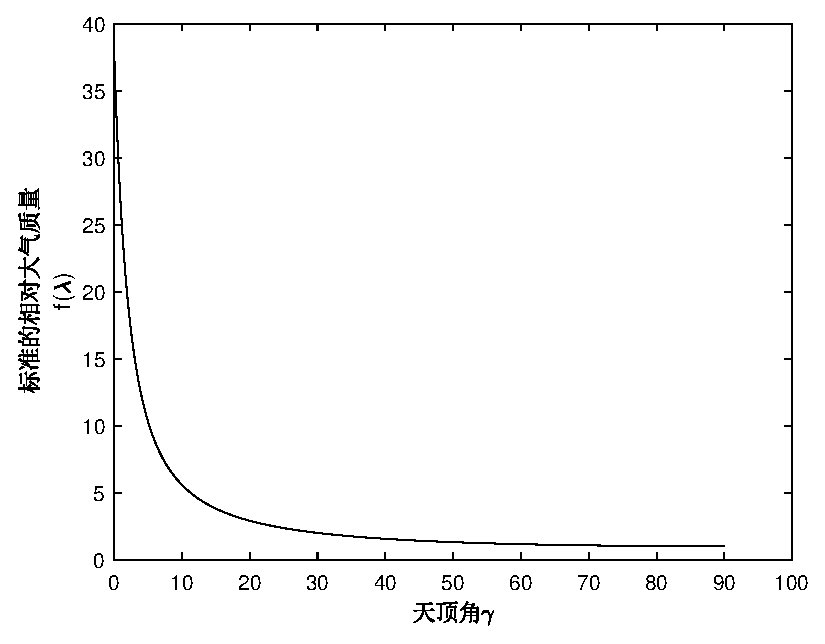
\includegraphics[width=16cm]{Standard.eps}
	\figcaption{标准的大气质量曲线}
\end{center}
\begin{center}
	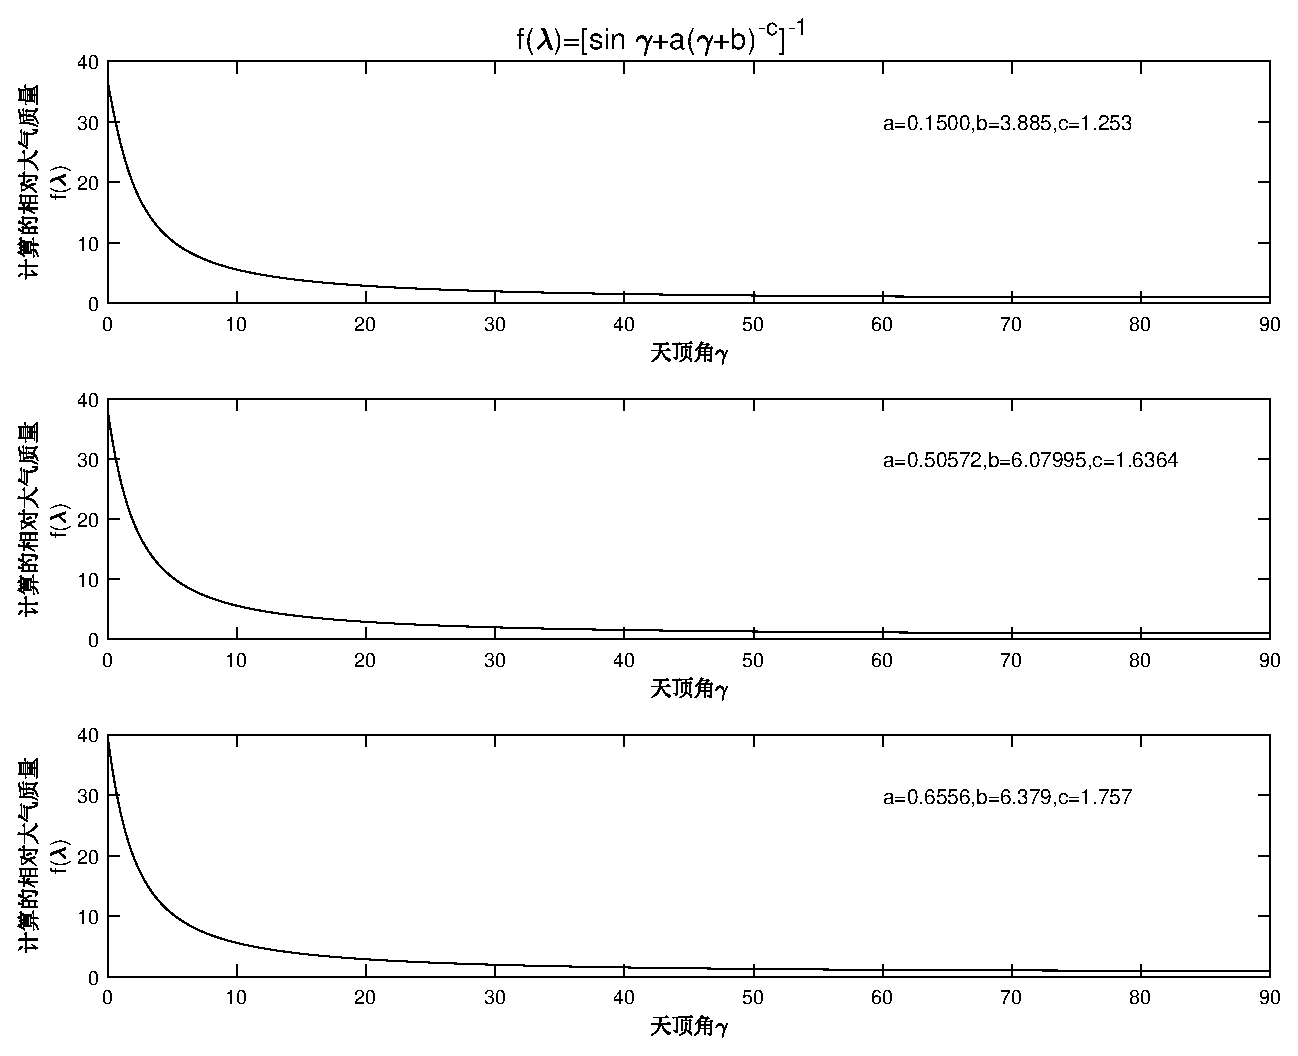
\includegraphics[width=16cm]{Calculate.eps}
	\figcaption{按照近似公式计算的大气质量曲线}
\end{center}
\begin{center}
	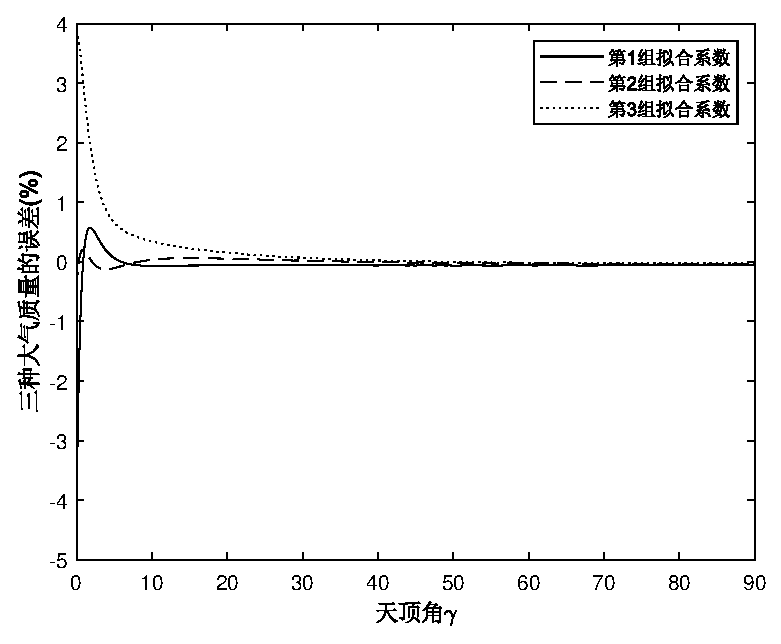
\includegraphics[width=16cm,height=9cm]{Error.eps}
	\figcaption{三种计算方法的误差曲线}
\end{center}

从上面的图中可以看到,用三种不同的系数计算的相对大气质量以及三组拟合系数的误差曲线,从图中可以看到,三者在天顶角大于30($^\circ$)之后都是差不多的经度,主要就是在30($^\circ$)之前的差异。而且可以看到在起始点的时候,第一组和第三组都有很大的误差,特别是第三组,误差都接近于4\%,回想文章中提到的积分会在$\gamma=0$和$h$接近于0的地方不定,需要查阅参考文献\upcite{bib:one}来寻找解决方法。但是我看到这个计算的第二组拟合系数表现的很好,不知道是否可以用第二组数据来计算,或者是这三组数据都是在不同的情况下表现的经度水平会不一样。
\section{参考文献}
\begin{thebibliography}{9}%宽度9
\bibitem{bib:one}Kasten,"A New Table and Approximation Formula for the Relative Optical Air Mass",Arch.Meteorol.Geophys.Bioklimatol.Ser.B 14,206-223(1965).
\bibitem{bib:two}R.A Miner,K.S.W.Chamption,and H.L.Pond,The ARDC Model Atmosphere,1959,Air Force Surveys in Geophysics 11(AFCRL,1959)
\bibitem{bib:three}F.Link and L.Neuzil,Table of Light Trajectories in the Terrestrial Atmosphere(Hermann,Paris,1969)
\bibitem{bib:four}D.E Snier and A. Goldman,Refractive Effects in Remote Sensing of Atmosphere with Infrared Transmission Spectroscopy,(Ballistic Research Labratories,June 1975)
\bibitem{bib:five}Y. M. Treve, New Values of the Optical Air Mass and the
Refraction and Comparison with Previous Tables," in Proceed-ings, Second Tropospheric Refraction Effects Technical ReviewMeeting, Technical Documentary Rep. ESD-TDR 64-103, May1964 (National Technical Information Service Order AD-442626), pp.5-391.
\bibitem{bib:six}International Organization for Standardization,Standard Atmosphere,International Standard ISO253(1972)
\bibitem{bib:seven}S.L.Valley,Handbook of Geophysics and Space Physics
(AFCRL,1965), pp.23.
\bibitem{bib:eight}W.H.Jefferys,M.J.Fitzpatrick,B.E.McArthur,andJ.E.
McCartney, GaussFit:A System for Least Squares and RobustEstimation (U. Texas at Austin, 1989).
\bibitem{bin:nine}A.T.Young,Observational Technique and Data Reduction," inle to Methods of Experimental Physics(Vol. 12, Astrophysics; Partrmly A:Optical and Infrared),N,Carleton,Ed.(Academic, New York, 1974),p.150.

\end{thebibliography}

\section{MATLAB代码}
主程序代码,用来调用三个近似计算公式,计算大气质量并且画图:
\lstinputlisting[language={MATLAB},
numbers=left, numberstyle={\normalsize },	commentstyle=\color{red!50!green!50!blue!50}, 
frame=shadowbox, rulesepcolor=\color{red!20!green!20!blue!20}]
{code/main.m}
三个近似计算公式如下:
\lstinputlisting[language={MATLAB},
numbers=left, numberstyle={\normalsize },	commentstyle=\color{red!50!green!50!blue!50}, 
frame=shadowbox, rulesepcolor=\color{red!20!green!20!blue!20}]
{code/massCal1.m}

\lstinputlisting[language={MATLAB},
numbers=left, numberstyle={\normalsize },	commentstyle=\color{red!50!green!50!blue!50}, 
frame=shadowbox, rulesepcolor=\color{red!20!green!20!blue!20}]
{code/massCal2.m}

\lstinputlisting[language={MATLAB},
numbers=left, numberstyle={\normalsize },	commentstyle=\color{red!50!green!50!blue!50}, 
frame=shadowbox, rulesepcolor=\color{red!20!green!20!blue!20}]
{code/massCal3.m}
\end{document} 